\subsection{CPU}

La primera qüestió a plantejar-nos ha estat quin seria el processador meś adient. Per a prendre una decisió de la forma més encertada possible, hem cregut oportú elaborar una taula amb diverses possibilitats i comparar les característiques de totes elles. Els principals criteris valorats per a prendre aquesta elecció, tal com es pot veure a la figura \ref{chartCPUs}, han estat els GFlops/Socket, els GFlops/Watt i els GFlops/Dòllar (sent els GFlops normalitzats respecte la mitjana). 

\begin{figure}[h]
    \centering
    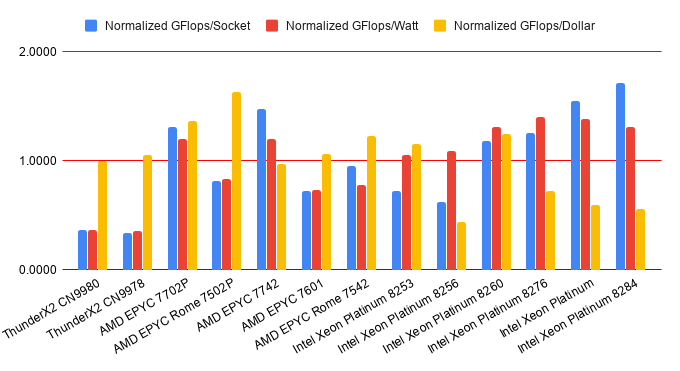
\includegraphics[width=\textwidth]{img/chartCPU}
    \caption{Comparativa entre les diverses CPUs valorades.}
    \label{chartCPUs}
\end{figure}

Després d'estudiar els resultats, per tenir un major marge de maniobre de cara a decisions futures hem pre-seleccionat dos processadors: l'\textit{AMD EPYC 7702P} \cite{cpu_amd_7702_buy} i l'\textit{AMD EPYC Rome 7502P} \cite{cpu_amd_7502_buy}, el primer per mostrar un excel·lent equilibri entre les tres principals característiques estudiades, i el segon per oferir el GFlop més barat sense menystenir excessivament els altres dos aspectes principals.